\section{Results}
\subsection{40 Minute Single Voxel Simulation}
\begin{frame}{Long Run Results}
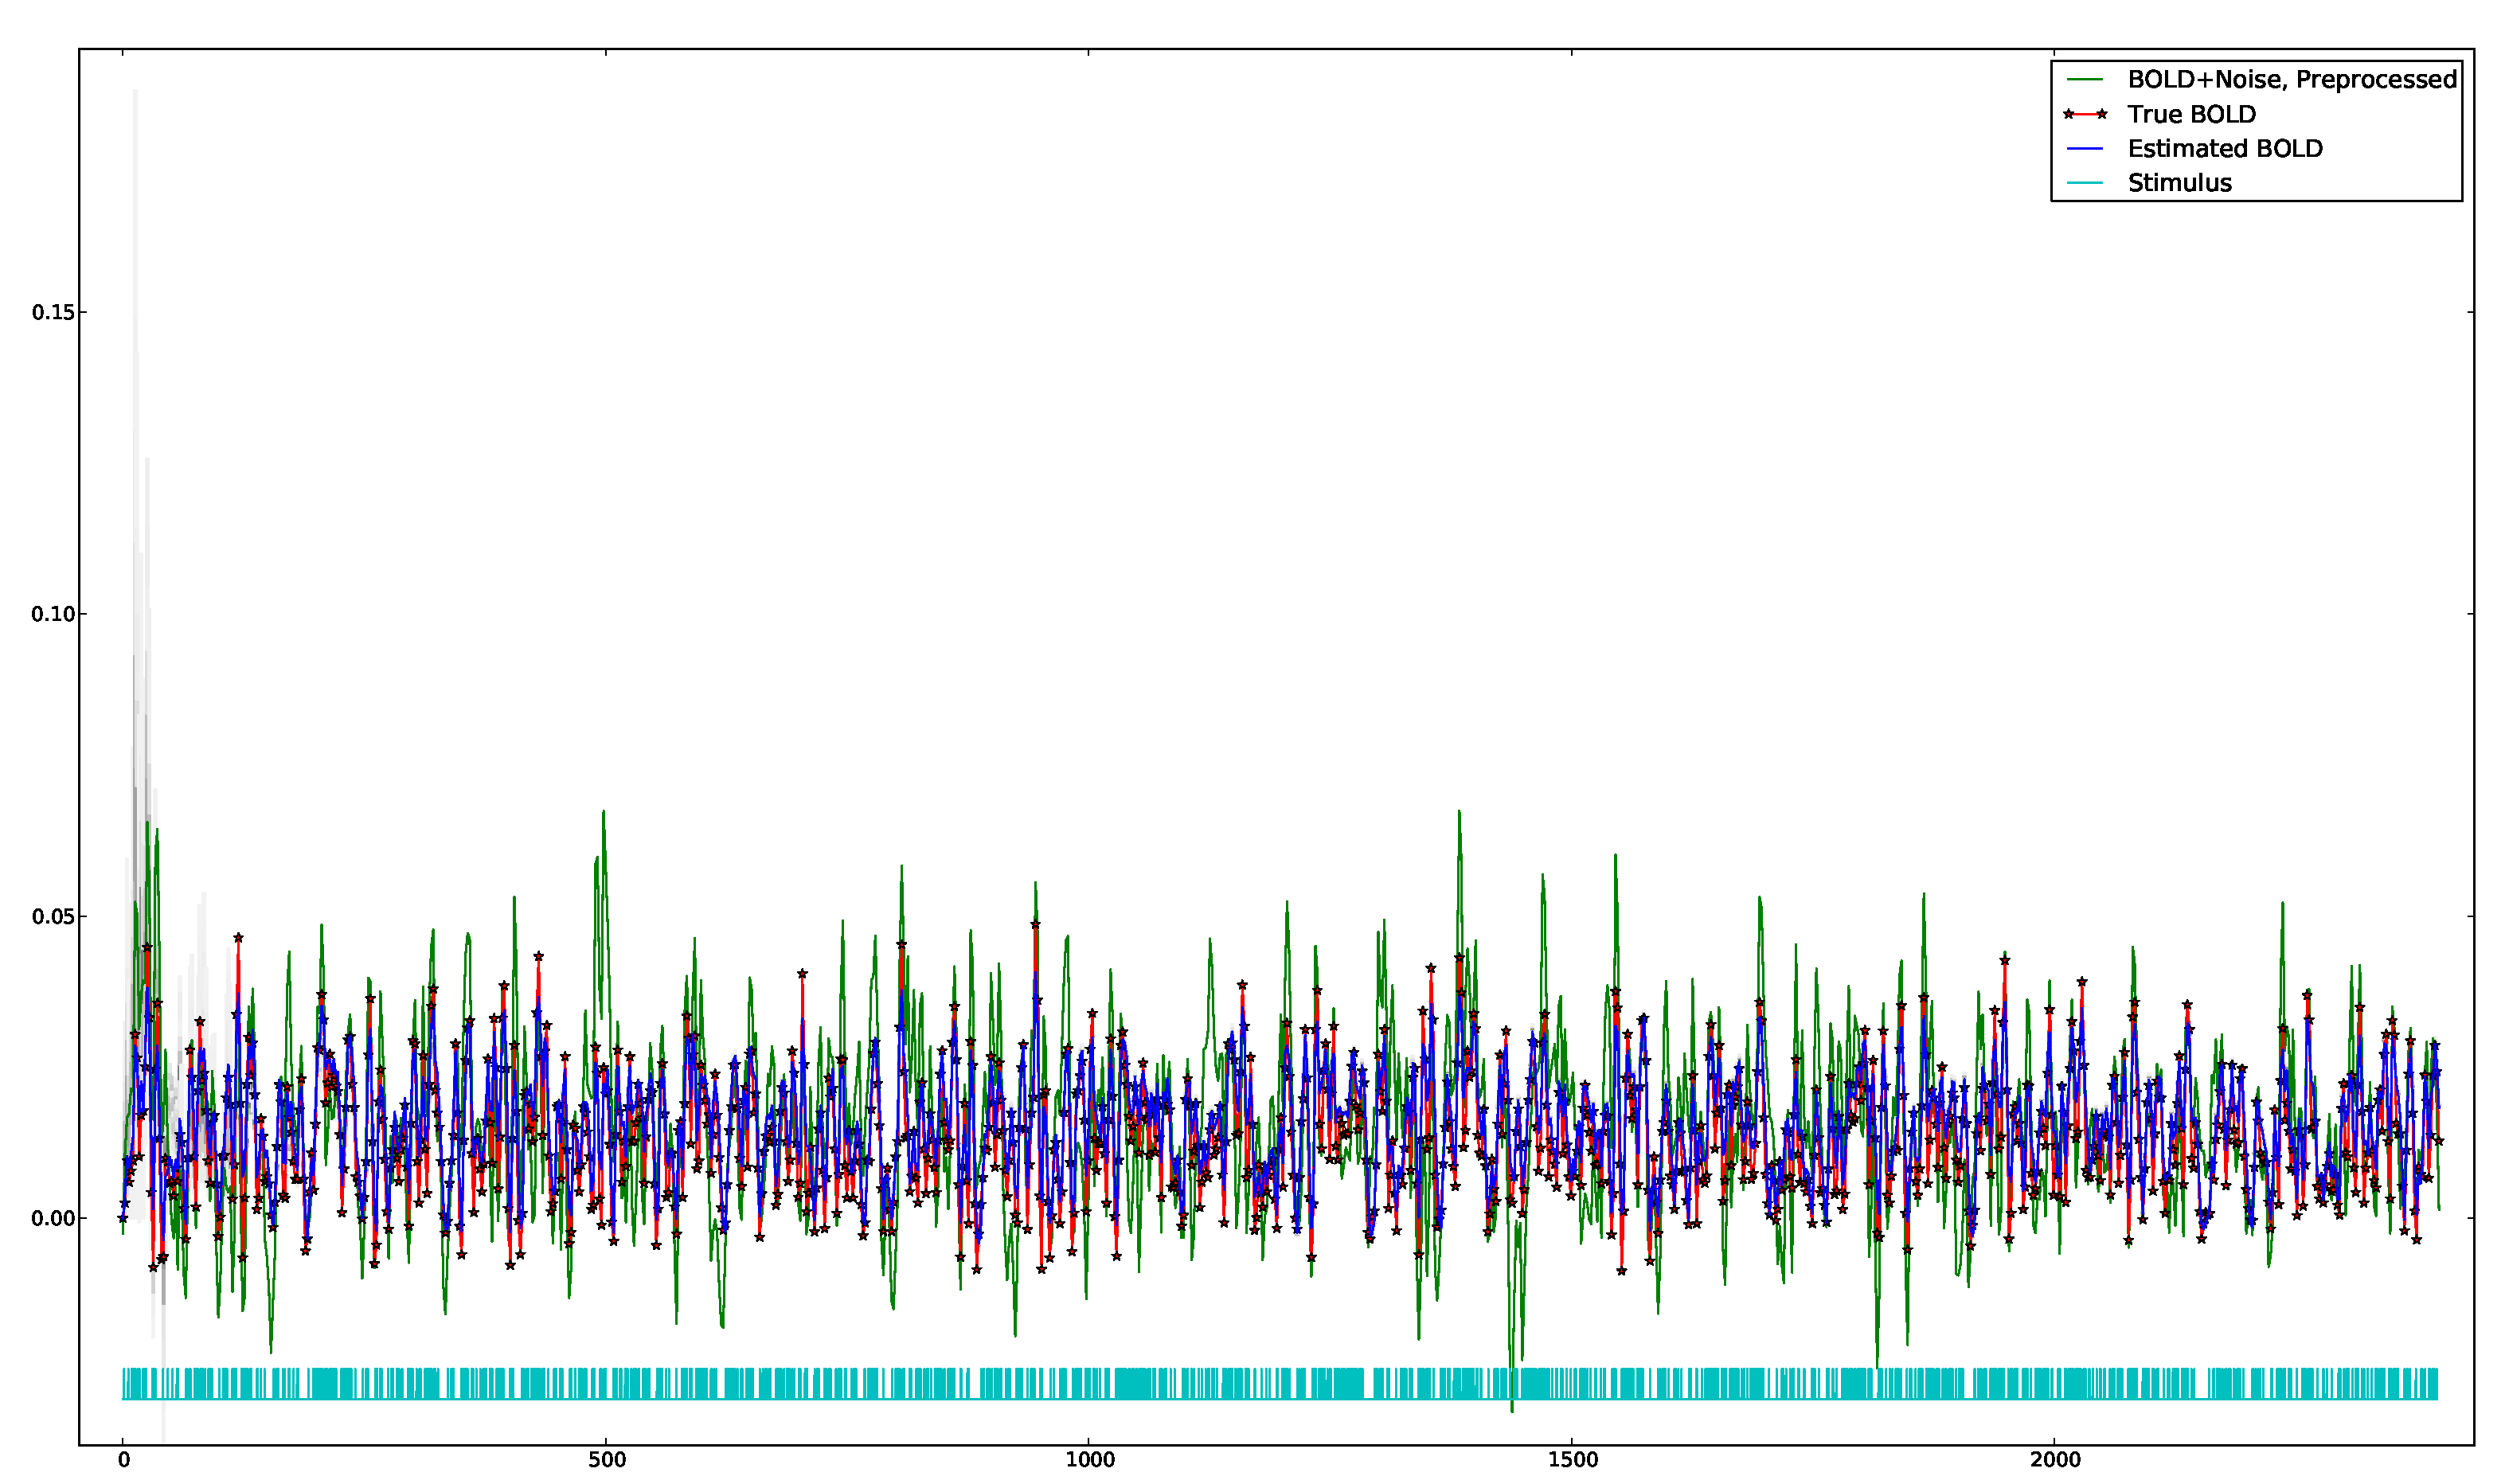
\includegraphics[width=\textwidth]{long_converge}
\note{
\begin{itemize}
\item Converge 250 measurements
\item Random spike stimulus, average 1 per second
\item Definitely excites system
\end{itemize}
}
\end{frame}

\begin{frame}{Long Run Covariance and Correlation}
\centering
Estimated Parameter Covariance 

\begin{table}[t]
\tiny
\begin{tabular}{|c | c  c  c  c  c  c  c |}
\hline
  & $\tau_0$ & $\alpha$ & $E_0$    & $V_0$    & $\tau_s$ & $\tau_f$ & $\epsilon$ \\
\hline
\rowcolor[gray]{.8} $\tau_0$  & 0.0004334 & 5.2e-05 & -6.95e-05 & 3.3e-06 & 0.0001628 & -2e-07 & 0.0001798 \\
$\alpha$                      & 5.2e-05 & 7.9e-06 & -6.4e-06 & 3e-07 & 1.04e-05 & -1.92e-05 & 2.58e-05 \\
\rowcolor[gray]{.8} $E_0$     & -6.95e-05 & -6.4e-06 & 1.9e-05 & -9e-07 & -4.11e-05 & -3.24e-05 & -3.92e-05 \\
$V_0$                         & 3.3e-06 & 3e-07 & -9e-07 & 1e-07 & 1.1e-06 & 9e-07 & 1e-06 \\
\rowcolor[gray]{.8} $\tau_s$  & 0.0001628 & 1.04e-05 & -4.11e-05 & 1.1e-06 & 0.0001589 & 0.0001518 & 7.88e-05 \\
$\tau_f$                      & -2e-07 & -1.92e-05 & -3.24e-05 & 9e-07 & 0.0001518 & 0.0002966 & -2.34e-05 \\
\rowcolor[gray]{.8} $\epsilon$& 0.0001798 & 2.58e-05 & -3.92e-05 & 1e-06 & 7.88e-05 & -2.34e-05 & 0.0001966 \\
\hline
\end{tabular}
\label{tab:long_cov}
\end{table}

Estimated Parameter Correlation 

\begin{table}[t]
\tiny
\begin{tabular}{|c | c  c  c  c  c  c  |}
\hline
  & $\tau_0$ & $\alpha$ & $E_0$    & $V_0$    & $\tau_s$ & $\tau_f$  \\
\hline
\rowcolor[gray]{.8} $\tau_0$  & & & & & & \\
$\alpha$                      & 0.889884 & & & & & \\
\rowcolor[gray]{.8} $E_0$     & -0.7661395 & -0.5230723 & & & & \\
$V_0$                         & 0.6244049 & 0.4239271 & -0.7964774 & & & \\
\rowcolor[gray]{.8} $\tau_s$  & 0.6204843 & 0.295425 & -0.7481253 & 0.3440421 & & \\
$\tau_f$                      & -0.0004259 & -0.3966881 & -0.4314174 & 0.1962954 & 0.6990775 & \\
\rowcolor[gray]{.8} $\epsilon$& 0.6158116 & 0.6558179 & -0.641348 & 0.2846632 & 0.4458142 & -0.097079 \\
\hline
\end{tabular}
\label{tab:long_corr}
\end{table}
\note{
\begin{itemize}
\item Covariance and Correlation of the run from the last slide
\item Significant correlation in parameters that don't change with time
\item very favorable situation, long with random stimulus, low noise
\item Not the fault of the particle filter b/c it gives good estimate
        of the BOLD signal
\end{itemize}
}
\end{frame}

\subsection{5 Minute, Single Voxel Simulation}
\begin{frame}{Preprocessed Noisy Simulation vs. Underlying Signal}
\begin{center}
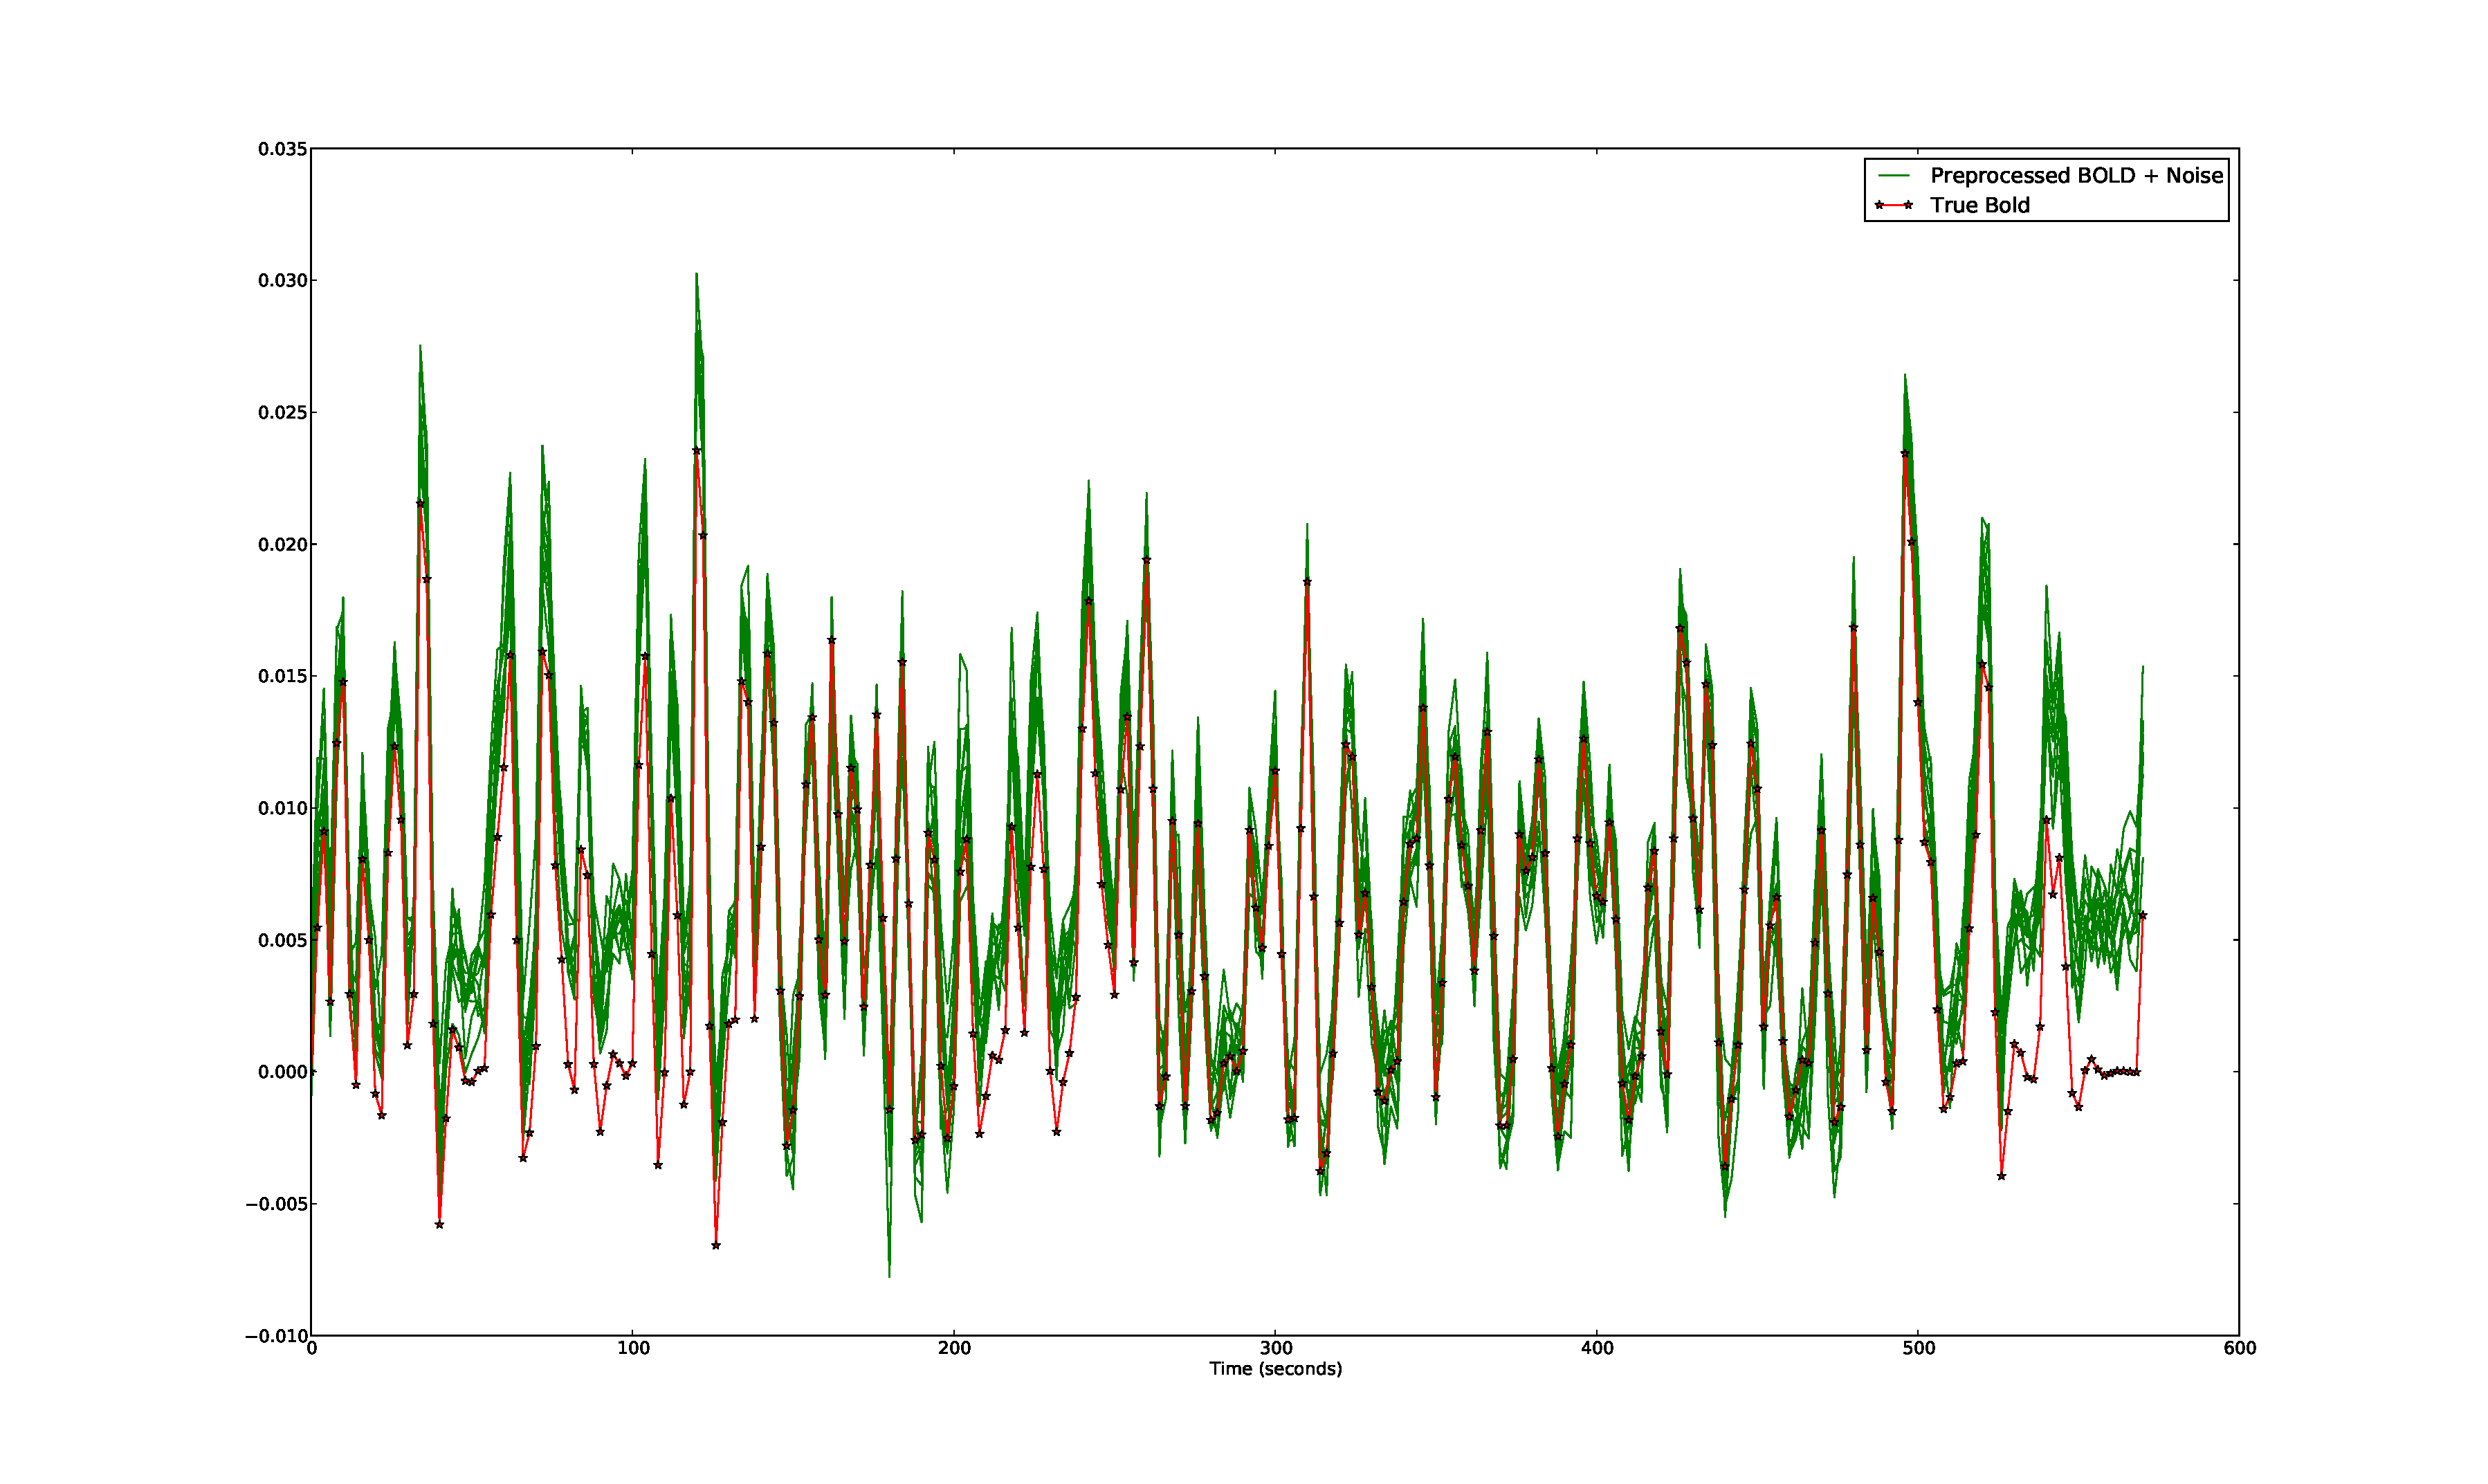
\includegraphics[clip=true,trim=6cm 2cm 5cm 3.5cm,width=.9\textwidth]
            {preprocessed_lownoise}
\end{center}
\note{
\begin{itemize}
\item Simulation with $0.001$, $0.0005$, SNR of about 10
\item the Drift has been mostly removed
\item 100 seconds, end still structure to noise
\end{itemize}
}
\end{frame}

\begin{frame}{Estimated vs. Underlying Signal}
\begin{center}
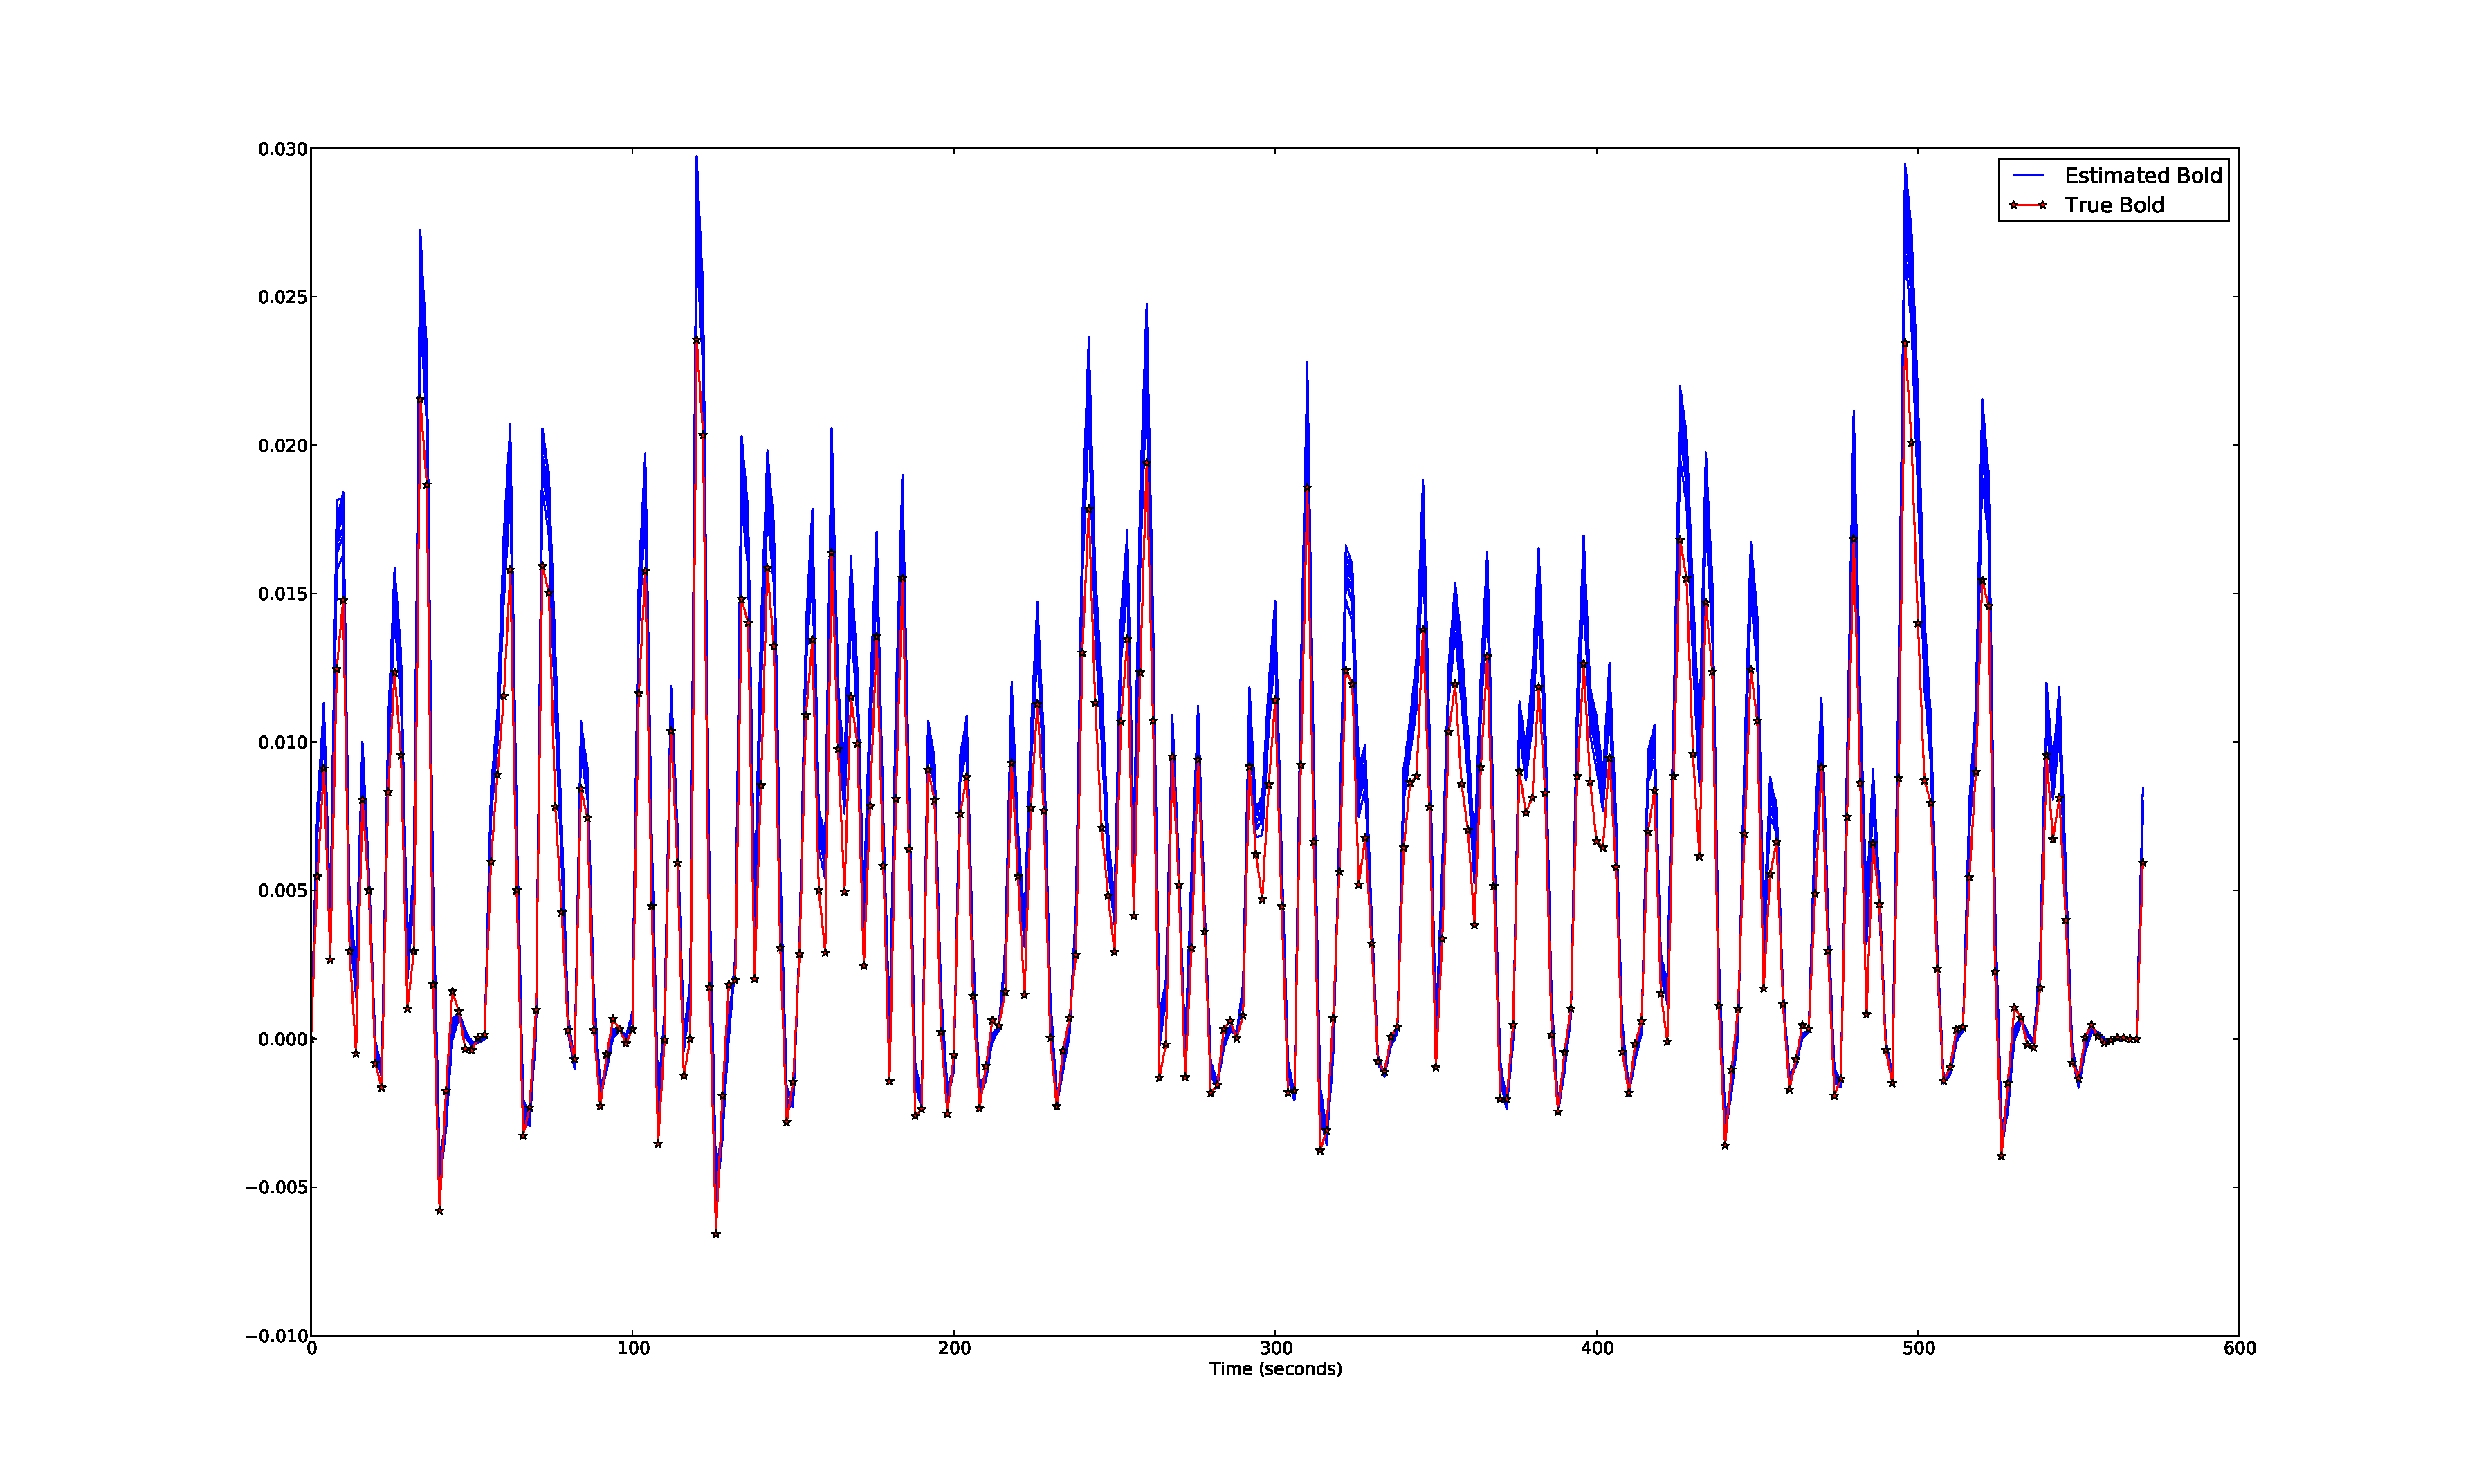
\includegraphics[clip=true,trim=6cm 2cm 5cm 3.5cm,width=.9\textwidth]
            {comparison_lownoise}
\end{center}
\note{
\begin{itemize}
\item Results from previous simulation
\item Note how well the estimates fit, in spite of drift at 100s, end
\end{itemize}
}
\end{frame}

\begin{frame}{Estimated Parameters}
\begin{table}[t]
\centering
\resizebox{\textwidth}{!}{
\begin{tabular}{|c | c | c | c | c | c | c | c | c | c |}
\hline
$\tau_0$ & $\alpha$ & $E_0$    & $V_0$    & $\tau_s$ & $\tau_f$ & $\epsilon$  & $ \sum \tau $ & Residual & Error\\
\hline
\rowcolor[gray]{.8}
1.45 & 0.3 & 0.47 & 0.044 & 1.94 & 1.99 & 1.8  & 5.38 &  & \\
\hline
\hline
1.2221 & 0.3449 & 0.3346 & 0.0714 & 1.6045 & 2.2753 & 1.5945 & 5.1019 &  0.003211  & 0.00224\\
1.3749 & 0.3318 & 0.3630 & 0.0733 & 1.6408 & 2.1030 & 1.5763 & 5.1187 &  0.003055  & 0.00223\\
1.1660 & 0.3221 & 0.3406 & 0.0822 & 1.6477 & 2.3535 & 1.2452 & 5.1672 &  0.003289  & 0.00205\\
1.2318 & 0.3271 & 0.3403 & 0.0796 & 1.6270 & 2.1852 & 1.3033 & 5.0439 &  0.002847  & 0.00147\\
1.1832 & 0.3179 & 0.3472 & 0.0821 & 1.5496 & 2.2912 & 1.2782 & 5.0240 &  0.003006  & 0.00213\\
1.1424 & 0.334  & 0.3473 & 0.0737 & 1.6221 & 2.2908 & 1.4025 & 5.0553 &  0.002833  & 0.00184\\
1.3004 & 0.3596 & 0.3564 & 0.0768 & 1.5641 & 2.1323 & 1.6034 & 4.9968 &  0.003028  & 0.00255\\
1.2401 & 0.3460 & 0.3398 & 0.0891 & 1.6499 & 2.2366 & 1.2900 & 5.1265 &  0.003044  & 0.00238\\
1.1709 & 0.3274 & 0.3464 & 0.0826 & 1.5373 & 2.2826 & 1.3783 & 4.9909 &  0.003345  & 0.0027 \\
1.1897 & 0.3434 & 0.3355 & 0.0798 & 1.5358 & 2.3075 & 1.4277 & 5.0330 &  0.003175  & 0.00244\\
1.184 &  0.3405 & 0.3502 & 0.0892 & 1.6103 & 2.2793 & 1.1645 & 5.0735 &  0.002889  & 0.00188\\
\hline                                                                               
1.2187 & 0.3359 & 0.3456 & 0.0800 & 1.599 & 2.2488 & 1.3876 & 5.0665 & 0.003066     & 0.00217\\
\hline
\end{tabular}
}
\end{table}
\note{
\begin{itemize}
\item Parameter estimates from previous simulation
\item Significant swings in parameters
\item Error is less than residual, meaning came closer to true signal than it
        did to the noisy signal.
\end{itemize}
}

\end{frame}

\subsection{POSSUM Simulation}
\begin{frame}{Mutual Information Compared with SNR}
\begin{figure}
\centering
\subfigure[Regions]{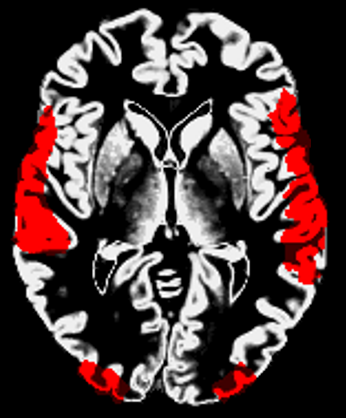
\includegraphics[height=.46\textheight]{simregions}}
\subfigure[Mutual Information]
{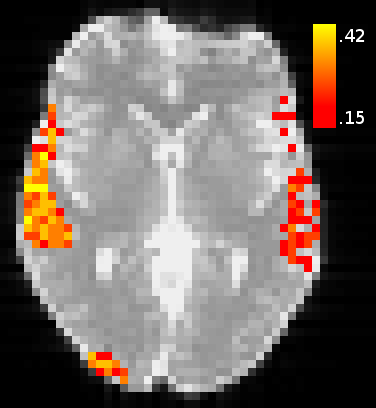
\includegraphics[height=.46\textheight]{sim_hm_15_6}}
\subfigure[SNR]{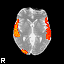
\includegraphics[height=.46\textheight]{snr_hm}}
\end{figure}
\note{
    \begin{itemize}
    \item A full slice simulated using Physics Oriented Simulated Scanner 
            For Understanding MRI (POSSUM)
    \item Each of 5 regions was given a distinct parameter set
    \item Noise is modeled realistically
    \item White matter, grey matter, and CSF treated differently
    \item Mean SNR's Region 1: $0.8$, Region 2: $0.97$, and Region 3: $0.39$.
    \item Regions 1 and 2 stick out. 
    \end{itemize}
}
\end{frame}

\begin{frame}{Mutual Information Compared with SNR, with threshold}
\begin{figure}
\centering
\subfigure[Regions]{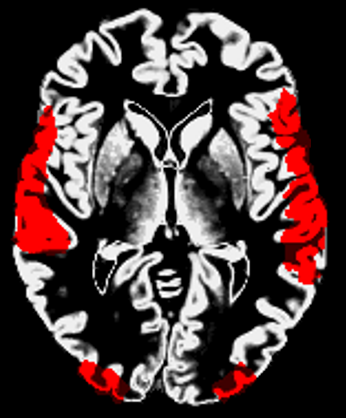
\includegraphics[height=.46\textheight]{simregions}}
\subfigure[Mutual Information]
{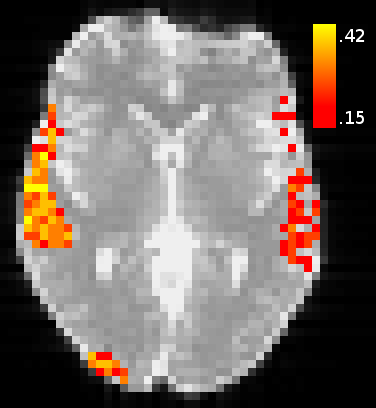
\includegraphics[height=.46\textheight]{sim_hm_15_6}}
\subfigure[SNR]{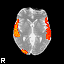
\includegraphics[height=.46\textheight]{snr_hm}}
\end{figure}
\note{
    \begin{itemize}
        \item In order to build histograms of the parameters in each
            region, I only used successful voxels, based on M.I.
        \item Requires threshold
        \item If a region does not correlate with the input, 
            parameters can't be found.
    \end{itemize}
}
\end{frame}

\begin{frame}{POSSUM Results: Histogram}
\begin{figure}
%\centering
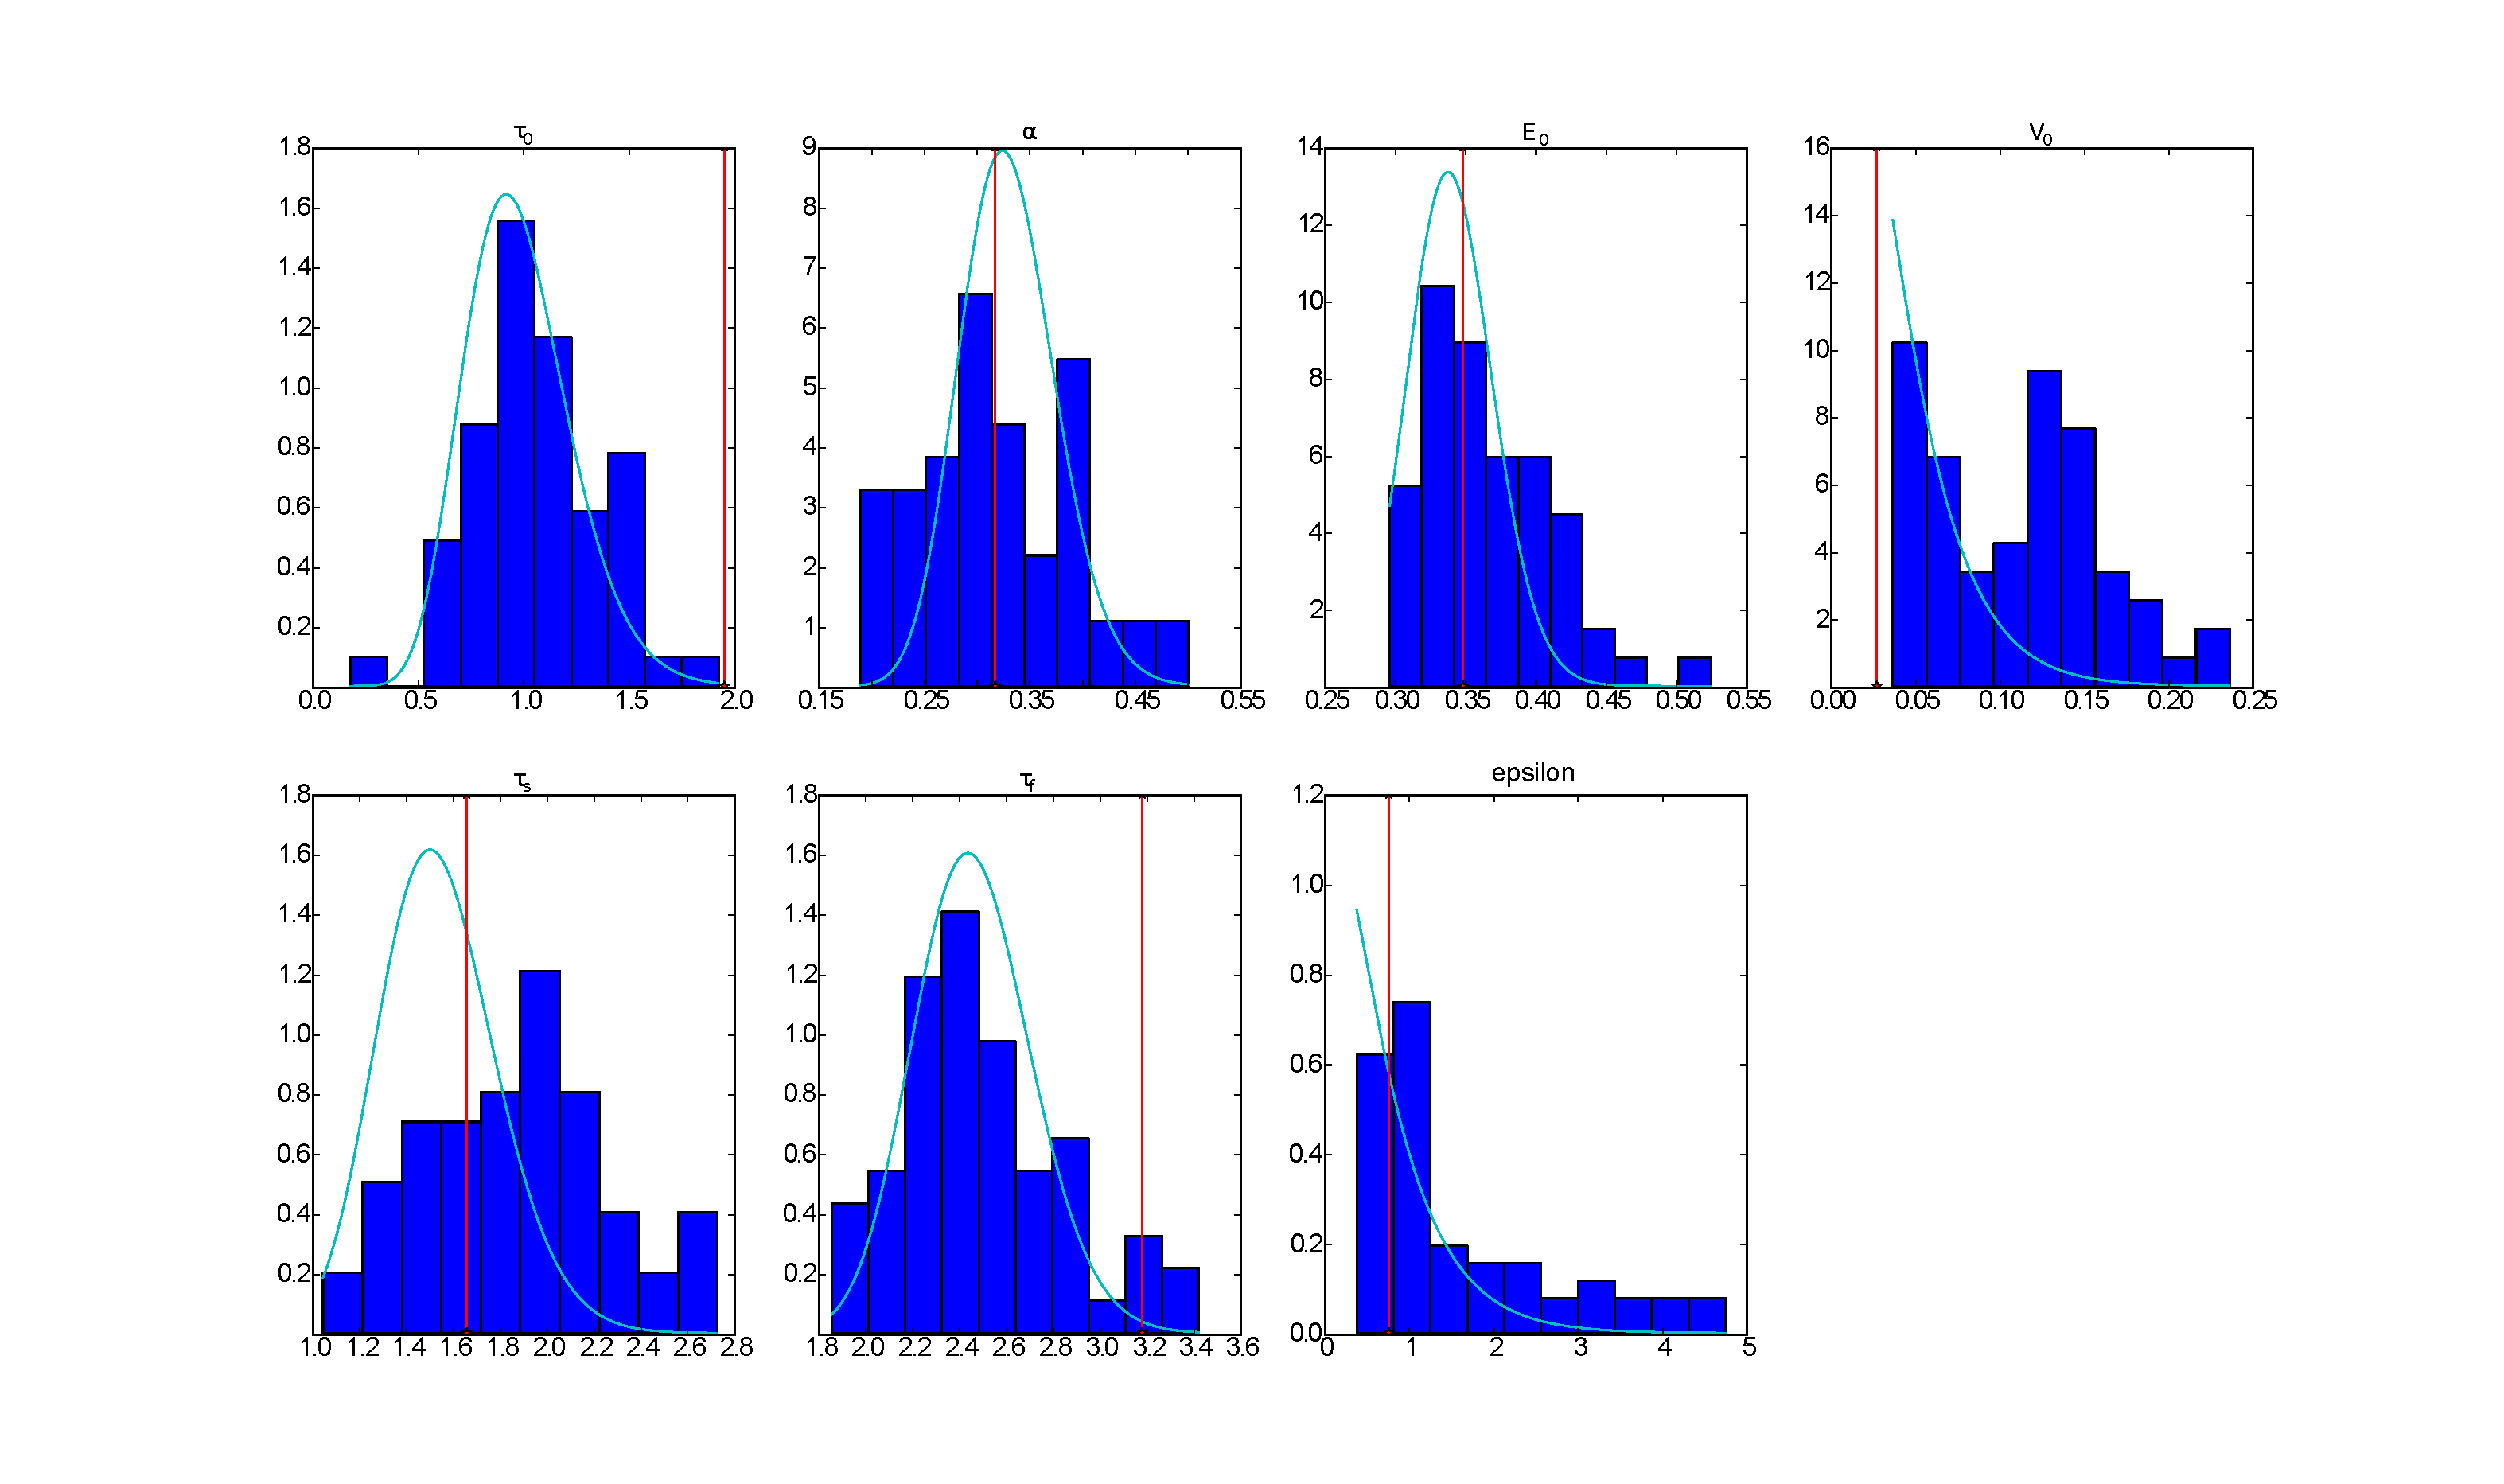
\includegraphics[clip=true,trim=5cm 2cm 5cm 2cm, width=.9\textwidth]{sec2hist}
\end{figure}
\note{
\begin{itemize}
\item Histogram of estimated parameters.
\item These estimates are all the mean
\item large variance
\item In spite of "good" fit, many parameter did not move far from prior
\end{itemize}
}
\end{frame}

\subsection{Real FMRI Data}
\begin{frame}{SPM vs. Mutual Information Map}
\begin{columns}
\begin{column}{.5\textwidth}
\begin{figure}
\setcounter{subfigure}{0}

\subfigure[SPM Results]{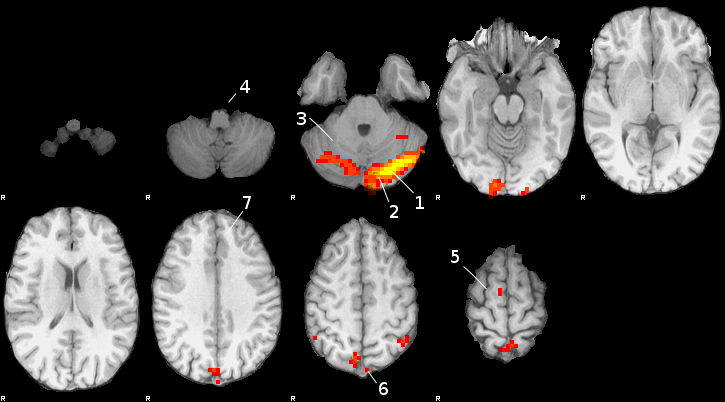
\includegraphics[width=.9\textwidth]{spm_hm}}
\subfigure{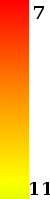
\includegraphics[width=.07\textwidth]{scale1}}
\label{fig:hm_canon_spm}
\end{figure}
\end{column}

\begin{column}{.5\textwidth}
\begin{figure}
\setcounter{subfigure}{1}
\subfigure[Particle Filter Results]{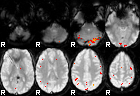
\includegraphics[width=.9\textwidth]{hm_mi_strict}}
\subfigure{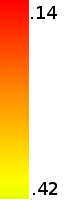
\includegraphics[height=1.5cm,width=.07\textwidth]{scale4}}
\end{figure}
\end{column}
\end{columns}
\note{
\begin{itemize}
\item Explain Units
\item Many of the regions agree
\item Definite areas of disagreement
\item There are several causes for the disagreement
\begin{itemize}
    \item SPM smooths quite heavily, 
    \item removes small regions of moderate activation
    \item Spreads out some regions of high activation
    \item SPM is not adaptable, so definite false negatives
    \item My algorithm could definitely have false positives and false negatives.
    \item Mutual Information isn't perfect
\end{itemize}
\end{itemize}
}
\end{frame}

\begin{frame}{Particle Filter Results: Histogram}
\begin{figure}
\centering
\includegraphics[width=.95\textwidth]{realhistm}
\end{figure}
\note{
\begin{itemize}
\item Histogram of parameters in active regions ($M.I. > .15$).
\item Mean from other works shown by red line.
\end{itemize}
\begin{table}[t]
\centering
\begin{tabular}{|c || c | c |}
\hline 
Parameter  & Friston et al. \cite{Friston2002} & Jonston et al. \cite{Johnston2008}\\ 
    
\hline
$\tau_0  $ &  $N(.98 , .25^2)$  & $8.38 \pm 1.5  $ \\
$\alpha  $ &  $N(.33 , .045^2)$  & $.189 \pm .004$ \\
$E_0     $ &  $N(.34 , .1 ^2)$  & $.635 \pm .072 $ \\
$V_0     $ &  $.03$ (NC)        & $.0149 \pm .006$ \\
$\tau_s  $ &  $N(1.54, .25^2)$  & $4.98 \pm 1.07 $ \\
$\tau_f  $ &  $N(2.46, .25^2)$  & $8.31 \pm 1.51 $ \\
$\epsilon$ &  $N(.54 , .1 ^2)$  & $.069 \pm .014 $ \\
\hline
\end{tabular}
\end{table}
}
\end{frame}

